\documentclass[a4paper,12pt]{article}
\usepackage{graphicx}
\usepackage{amsmath}
\usepackage[margin=1in]{geometry}
\usepackage{amsmath, amssymb}
\usepackage{float}
\usepackage{caption}
\usepackage{subcaption}
\usepackage{xcolor}
\usepackage{fancyhdr}
\usepackage{array}
\usepackage{float}

\geometry{a4paper, top=0.7in, left=1in, right=1in, bottom=1in}

\begin{document}
\thispagestyle{fancy}
\fancyhf{} 
\renewcommand{\headrulewidth}{0pt} 

\fancyhead[L]{
        
\includegraphics[width=8cm, height=1.7cm]{comet.jpeg} 
        }
\fancyhead[R]{
    Name: G.MADHU LATHA \\
    Batch: COMETFWC029\\
    Date: 21-may 2025
}
\vspace{1cm}
\begin{center}
    {\LARGE \textbf{\textcolor{black}{\\  GATE QUESTION \\ ECE 2009 Q53}}}
\end{center}
\vspace{-1cm}
\section*{\textcolor{cyan}{ \\Question :}}
\textbf{Q58)The following Karnaugh map represents a function F:} \\
\vspace{1em}
\begin{center}
\begin{minipage}[t]{0.38\textwidth}
\vspace{-3em}
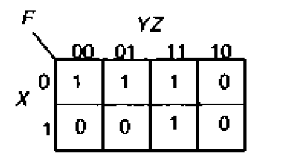
\includegraphics[height=5cm,width=\linewidth]{task31.png}

\end{minipage}
\end{center}
\vspace{0.5em}
\textbf{Which of the following circuits is a realization of the above function F?}
\begin{center}
\begin{minipage}[t]{1\textwidth}
\vspace{-1.5em}
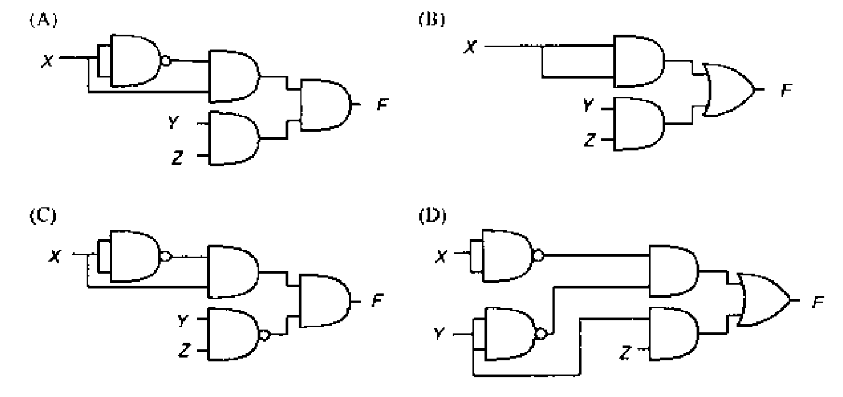
\includegraphics[height=6cm,width=\linewidth]{task32.png}

\end{minipage}
\end{center}
 \section*{\textcolor{cyan}{Solution:}}
 
\textbf{Given K-map:} \\
From this K-map, the minterms where \( F = 1 \) are:
\begin{enumerate}
    \item \( m_0 \): \( X = 0, Y = 0, Z = 0 \Rightarrow \overline{X} \, \overline{Y} \, \overline{Z} \)
    \item \( m_1 \): \( X = 0, Y = 0, Z = 1 \Rightarrow \overline{X} \, \overline{Y} \, Z \)
    \item \( m_7 \): \( X = 1, Y = 1, Z = 1 \Rightarrow X Y Z \) \\
\end{enumerate}
Given K-map is 
\begin{center}
\begin{minipage}[t]{0.38\textwidth}
\vspace{-3em}
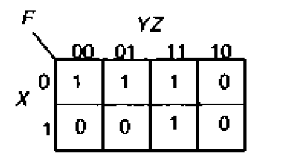
\includegraphics[height=5cm,width=\linewidth]{task31.png}
\end{minipage}
\end{center}

So, the Boolean expression is:
\[
F = \overline{X} \, \overline{Y} \, \overline{Z} + \overline{X} \, \overline{Y} \, Z + X Y Z
\]

Group the first two terms:
\[
F = \overline{X} \, \overline{Y} (\overline{Z} + Z) + X Y Z = \overline{X} \, \overline{Y} + X Y Z
\]

So the correct simplified form is:
\[
\boxed{F = \overline{X} Y + Y Z}
\]

\textbf{Now examining the circuits in Q.53:}

\textbf{Figure 1:} performs the following operations:
\begin{enumerate}
    \item First, invert \( X \) to get \( \overline{X} \)
    \item AND gate: \( \overline{X} \cdot Y = \overline{X} Y \)
    \item AND gate: \( Y \cdot Z = Y Z \)
    \item OR gate: \( \overline{X} Y + Y Z \)
\end{enumerate}
\textbf{This matches the simplified function.}

\section*{Final Answer:}
\[
\boxed{\text{Option (A)}}
\]

\end{document}
\end{document}
